\documentclass{article}

% Language setting
% Replace `english' with e.g. `spanish' to change the document language
% \usepackage[english]{babel}

% Set page size and margins
% Replace `letterpaper' with `a4paper' for UK/EU standard size
\usepackage[letterpaper,top=2cm,bottom=2cm,left=3cm,right=3cm,marginparwidth=1.75cm]{geometry}
% Useful packages
\usepackage{amsmath}
\usepackage{amssymb}
\usepackage{graphicx}
\usepackage{lineno}
% \usepackage{showkeys}
\usepackage[colorlinks=true, allcolors=blue]{hyperref}

\title{Your Paper}
\author{You}

\begin{document}
\maketitle

\begin{abstract}
Your abstract.
\end{abstract}

\linenumbers

\section{Introduction}

- source: 10.3389/fdgth.2024.1455446

One of the factors that affects the quality and cost of care is
patient flow, which refers to the efficient use of resources and
time during the patient’s stay in the hospital (9, 10). A common
practice for planning the discharge of patients is to rely on the
clinicians’ estimates of the discharge date. However, this practice
has some drawbacks, such as consuming the clinicians’ time that
could be spent on other tasks or direct patient care, and having
low accuracy (11, 12). A possible alternative is to apply machine
learning models to predict the discharge date of patients based
on their length of stay (LOS) in the hospital. Several studies have
proposed and developed different LOS models for this purpose
(11, 13–18).


% \section{Some examples to get started}

% \subsection{How to create Sections and Subsections}

% Simply use the section and subsection commands, as in this example document! With Overleaf, all the formatting and numbering is handled automatically according to the template you've chosen. If you're using the Visual Editor, you can also create new section and subsections via the buttons in the editor toolbar.

% \subsection{How to include Figures}

% First you have to upload the image file from your computer using the upload link in the file-tree menu. Then use the includegraphics command to include it in your document. Use the figure environment and the caption command to add a number and a caption to your figure. See the code for Figure \ref{fig:frog} in this section for an example.

% Note that your figure will automatically be placed in the most appropriate place for it, given the surrounding text and taking into account other figures or tables that may be close by. You can find out more about adding images to your documents in this help article on \href{https://www.overleaf.com/learn/how-to/Including_images_on_Overleaf}{including images on Overleaf}.

% \begin{figure}
% \centering
% 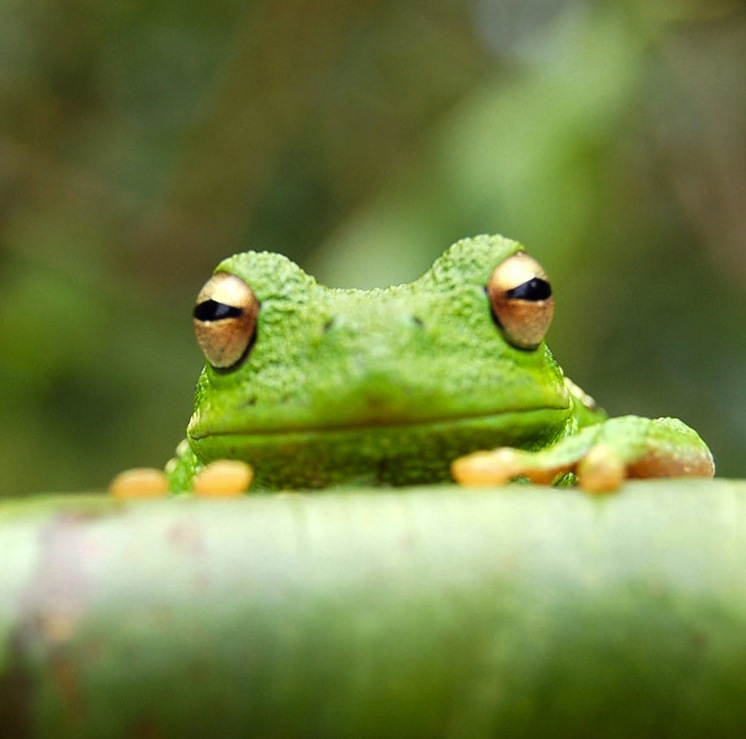
\includegraphics[width=0.25\linewidth]{frog.jpg}
% \caption{\label{fig:frog}This frog was uploaded via the file-tree menu.}
% \end{figure}

% \subsection{How to add Tables}

% Use the table and tabular environments for basic tables --- see Table~\ref{tab:widgets}, for example. For more information, please see this help article on \href{https://www.overleaf.com/learn/latex/tables}{tables}. 

% \begin{table}
% \centering
% \begin{tabular}{l|r}
% Item & Quantity \\\hline
% Widgets & 42 \\
% Gadgets & 13
% \end{tabular}
% \caption{\label{tab:widgets}An example table.}
% \end{table}

% \subsection{How to add Comments and Track Changes}

% Comments can be added to your project by highlighting some text and clicking ``Add comment'' in the top right of the editor pane. To view existing comments, click on the Review menu in the toolbar above. To reply to a comment, click on the Reply button in the lower right corner of the comment. You can close the Review pane by clicking its name on the toolbar when you're done reviewing for the time being.

% Track changes are available on all our \href{https://www.overleaf.com/user/subscription/plans}{premium plans}, and can be toggled on or off using the option at the top of the Review pane. Track changes allow you to keep track of every change made to the document, along with the person making the change. 

% \subsection{How to add Lists}

% You can make lists with automatic numbering \dots

% \begin{enumerate}
% \item Like this,
% \item and like this.
% \end{enumerate}
% \dots or bullet points \dots
% \begin{itemize}
% \item Like this,
% \item and like this.
% \end{itemize}

% \subsection{How to write Mathematics}

% \LaTeX{} is great at typesetting mathematics. Let $X_1, X_2, \ldots, X_n$ be a sequence of independent and identically distributed random variables with $\text{E}[X_i] = \mu$ and $\text{Var}[X_i] = \sigma^2 < \infty$, and let
% \[S_n = \frac{X_1 + X_2 + \cdots + X_n}{n}
%       = \frac{1}{n}\sum_{i}^{n} X_i\]
% denote their mean. Then as $n$ approaches infinity, the random variables $\sqrt{n}(S_n - \mu)$ converge in distribution to a normal $\mathcal{N}(0, \sigma^2)$.


% \subsection{How to change the margins and paper size}

% Usually the template you're using will have the page margins and paper size set correctly for that use-case. For example, if you're using a journal article template provided by the journal publisher, that template will be formatted according to their requirements. In these cases, it's best not to alter the margins directly.

% If however you're using a more general template, such as this one, and would like to alter the margins, a common way to do so is via the geometry package. You can find the geometry package loaded in the preamble at the top of this example file, and if you'd like to learn more about how to adjust the settings, please visit this help article on \href{https://www.overleaf.com/learn/latex/page_size_and_margins}{page size and margins}.

% \subsection{How to change the document language and spell check settings}

% Overleaf supports many different languages, including multiple different languages within one document. 

% To configure the document language, simply edit the option provided to the babel package in the preamble at the top of this example project. To learn more about the different options, please visit this help article on \href{https://www.overleaf.com/learn/latex/International_language_support}{international language support}.

% To change the spell check language, simply open the Overleaf menu at the top left of the editor window, scroll down to the spell check setting, and adjust accordingly.

% \subsection{How to add Citations and a References List}

% You can simply upload a \verb|.bib| file containing your BibTeX entries, created with a tool such as JabRef. You can then cite entries from it, like this: \cite{greenwade93}. Just remember to specify a bibliography style, as well as the filename of the \verb|.bib|. You can find a \href{https://www.overleaf.com/help/97-how-to-include-a-bibliography-using-bibtex}{video tutorial here} to learn more about BibTeX.

% If you have an \href{https://www.overleaf.com/user/subscription/plans}{upgraded account}, you can also import your Mendeley or Zotero library directly as a \verb|.bib| file, via the upload menu in the file-tree.

\subsection{Context}

background information to set the stage for the research

----------------------------------------------------

    Iezzoni et al., Med Care, 1988 – severity adjustment for LOS and discharge status in Medicare patients.

    Severity matters—but it doesn’t tell the whole story. Even with detailed physiologic data, over 80\% of LOS variation remained unexplained. Hospitals can likely reduce pneumonia LOS through care-process changes (e.g., standardized clinical pathways, early mobilization, streamlined discharge). For policymakers, simple claims-based risk adjustment is inadequate when using LOS as a quality or efficiency metric.

    Across 11 different severity measures—ranging from claims-based comorbidity counts to physiology-based scores—only ~10-15\% of the variation in individual patients’ length of stay (LOS) was explained (trimmed data, R² ≈ 0.10–0.15).

-----------------------------------------------------

\subsection{State of the art}

review of the current research, findings, and technologies in the field


------------------------------



\subsection{Research gap}

Identifies gaps in existing research that the project aims to address


------------------------------

- source: 10.3389/fdgth.2024.1455446

The majority of published articles in healthcare machine learning
have failed to showcase successful implementations of proposed
models, resulting in a substantial gap between theoretical
concepts and practical applications. This underscores the pressing
need for practical research that addresses the entire life cycle of
predictive models, spanning from their initial conceptualization
to their effective integration into operational systems (19, 20).


\subsection{Study objective, scope and deliverables}

Clearly define what the research intends to accomplish, its limitations, and what you will deliver (e.g., findings, models, recommendations).

\section{Methodology}

 research design, methods, and approaches used in the study

    -------------------------------------------------------------

    Methodology
    This study followed a structured data science workflow, consisting of data cleaning, merging, exploratory analysis, and preparation for modeling. The methodology is summarized as follows:

    1. Laboratory Data Cleaning and Exploration
    The laboratory dataset, spanning approximately 16 years, was first loaded and inspected (1_data_cleaning_eda_lab.ipynb). Data cleaning steps included:

    Renaming columns for clarity and consistency.
    Handling missing values, especially in the numeric_result and text_result columns.
    Removing duplicate rows and implausible values (e.g., extreme outliers or placeholder values such as 9999.0).
    Filtering out irrelevant or auxiliary laboratory tests.
    Checking for and addressing negative values and other data quality issues.
    2. Clinical Data Cleaning and Exploration
    The clinical dataset was similarly processed (2_data_cleaning_eda_clinical.ipynb):

    Standardizing column names and formats.
    Handling missing or inconsistent entries.
    Removing duplicates and ensuring data integrity.
    Extracting relevant features for downstream analysis.
    3. Data Merging
    The cleaned laboratory and clinical datasets were merged on patient and case identifiers (3_merge_data.ipynb):

    Only cases with sufficient laboratory and clinical information were retained.
    A reference table of laboratory tests was created to facilitate feature selection.
    The merged dataset was saved for further analysis.
    4. Outlier Analysis
    Outlier detection and handling were performed to improve data quality (4_outlier_analysis.ipynb):

    Statistical methods and visualizations were used to identify extreme values in key variables.
    Outliers were either removed or capped, depending on their nature and impact.
    5. Exploratory Data Analysis (EDA) of Merged Data
    Comprehensive EDA was conducted on the merged dataset (5_eda_merged_data.ipynb):

    Descriptive statistics and visualizations (e.g., boxplots, barplots) were used to summarize patient demographics, laboratory results, and clinical outcomes.
    The distribution of length of stay (LOS) and discharge types was analyzed.
    Relationships between variables were explored to inform feature engineering and modeling.
    This methodology ensured a robust and reproducible pipeline for preparing the data for predictive modeling of hospital length of stay and discharge type. Each step was documented in the corresponding Jupyter notebook for transparency and reproducibility.

\section{Evaluation}

how I will assess or measure the effectiveness or success of the research

\subsection{Evaluation Methodology}
\subsection{Results}


\section{Conclusions}

\bibliographystyle{alpha}
\bibliography{sample}

\end{document}